\chapter{DIRAC - The Distributed Infrastructure with Remote Agent Control}
\label{chap:DIRAC}

The LHCb Collaboration \cite{LHCb} is running one of the four large experiments at the LHC particle 
collider at CERN, Geneva. The amount of data produced by the experiment
annually is so large that it requires development of a specialized system for the data reconstruction, simulation 
and analysis. The DIRAC project of the LHCb Collaboration was started to
provide such a system.\cite{Dir2} The developers were aiming to create a easy to run system, which would be able 
to seamlessly utilize the various heterogeneous computing resources available to the LHCb Collaboration, 
that can be run by only one production manager. 

The DIRAC software architecture is based on a set of distributed, collaborating services. Designed to have a
light implementation, DIRAC is easy to deploy, configure and maintain on a variety of platforms. Following
the paradigm of a Services Oriented Architecture (SOA)\cite{SOA}, DIRAC is lightweight, robust and scalable. 
One of the primary goals was to support various virtual organization with their specific needs: it supports well 
isolated plugable modules, where the organizations specific features can be located. It allows to construct
grids of up to several thousands processors by integrating diverse resources within its integrated Workload
Management System. The DIRAC Data Management components provide access to standard grid storage systems. 
The File Catalog options include the LCG File Catalog (LFC) as well as a simple DIRAC File Catalog discussed later. 

\subsection{DIRAC Architecture}
DIRAC components can be grouped in to four categories: 

\begin{description}

\item[Resources] \hfill \\
Because every grid middleware has to deal with a large number of different technologies, it needs its own 
interfaces for each of them. To this end DIRAC has a class of components called Resources,
which provides access to the available computing and storage facilities. 
Computing resources include individual PCs, computer farms, cloud resources and computing grids. Storage 
resources include storage elements with SRM interface \cite{SRM} and most of the popular data access 
protocols (gridftp, (s)ftp, http,...) are integrated as well\footnote{DIRAC does not provide its own complex 
storage element, it includes however a Storage Element service which yields access to disk 
storage managed by a POSIX compliant file system. This is sufficient for small deployments and development
purposes}.

\pagebreak

\item[Services] \hfill \\
The DIRAC system is built around a set of loosely coupled services that keep the system status and
help to carry out workload and data management tasks. The Services are passive components which
are only reacting to the requests of their clients, possibly contacting other services in order to
accomplish their tasks. Each service has typically a MySQL \cite{MySQL} database backend to store the state
information. The services accept incoming connections from various clients. These can be user interfaces,
agents or running jobs. 

\item[Agents] \hfill \\
Agents are light and easy-to-deploy software components built around a unified framework. They are active
components, usually running close to the corresponding services, watching for changes in the service states and 
reacting accordingly by initiating actions like job submission or result retrieval. 

\item[Interfaces] \hfill \\
The DIRAC functionality is exposed to the system developers and to the users in a variety of ways. 
	\begin{itemize}
		\item The DIRAC programming language is python, so the programming interfaces (APIs) are available in this 
			language
		\item For users the DIRAC functionality is available through a command line interface. Some subsystems 		
			have specialized shells to work with.
		\item DIRAC also provides a web interface suitable for monitoring and managing the system behavior.
	\end{itemize}

\end{description}

\subsection{DIRAC Framework}

DIRAC’s logic is built on top of basic services that provide transversal
functionality to DIRAC Systems \cite{DISET}. The set of basic services that form the core framework for
DIRAC are: 
\begin{itemize}

\item \textbf{DISET -- secure communication protocol}
	is the DIRAC secure transport layer. DISET was created by enhancing the XML-RPC
	protocol with a secure layer with GSI\footnote{Grid Security Infrastructure} compliant authentication mechanism 
	\cite{DISET2}. 	It takes care of all the communication needs between DIRAC components. 
	When secure connections are not needed communication is done using plain TCP/IP.
	
\item \textbf{Configuration System}
	is built to provide static configuration parameters to all the distributed DIRAC components. Being able to
	distribute the configuration is critical. When the configuration data is not available, 
	the systems cannot work. For maximum reliability it is organized as a single master service, where 
	all the parameter updates are done, and multiple read-only slave services, which are distributed geographically.

\item \textbf{Web Portal}
	is the standard way to present information to visitors. It provides authentication based on user grid
	credentials and user groups: ordinary users can see their jobs and have minimal interaction with
	them, administrators can change the global configuration in a graphical interface.
	All the monitoring and control tools of a DIRAC system are exported through the Web portal, 
	which makes them uniform for users working in different environments and on different platforms.
	
\item \textbf{Logging System}
	is a uniform logging facility for all the DIRAC components.

\item \textbf{Monitoring System}
	collects activity reports from all the DIRAC services and some agents. Together
	with the Logging Service, it provides a complete view of the status of the system for the managers.
\end{itemize}
\begin{figure}[b]
	\centering
	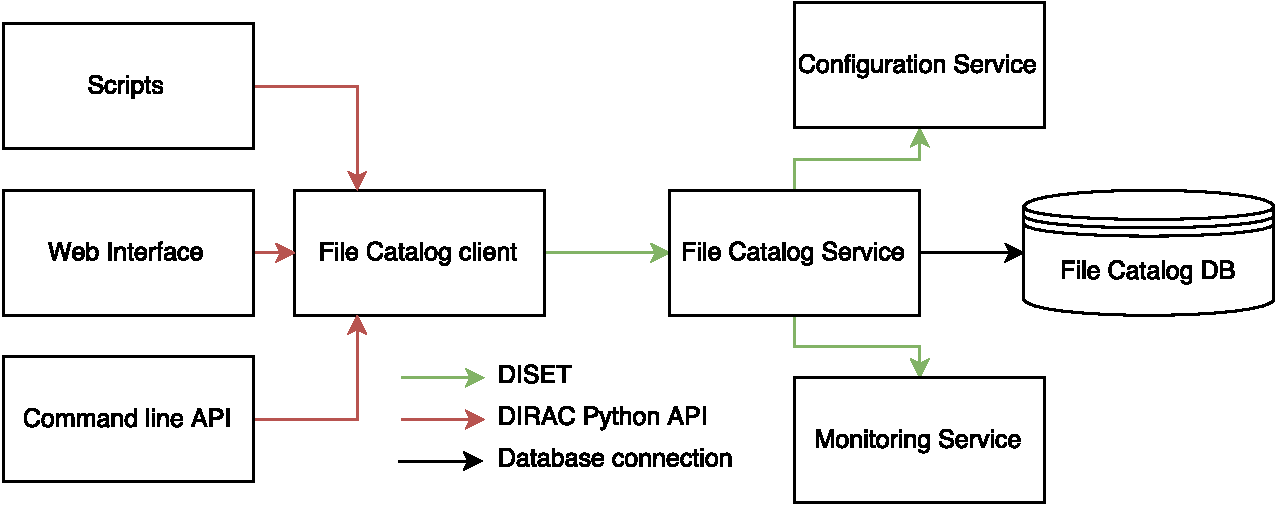
\includegraphics[width=\textwidth]{FileCatalogDiagramHor.pdf}
	\caption{DIRAC File Catalog built inside the DISET framework}
	\label{fig:FCDiag}
\end{figure}

Other widely used systems include the Workload Management System, able to manage simultaneously computing
tasks for a given user community \cite{WMS}, Request Management System \cite{RMS} managing simple operations, that 
are performed asynchronously on behalf of users, and others. 

\section{DIRAC Data Management System}

The DIRAC middleware solution covers the whole range of tools to handle data management tasks. The low level 
tools include many clients for various types of storage. In addition to providing clients of all 
the common storage systems, DIRAC also implements its own simple Storage Element. Both technologies are 
exposed to the users by a uniform API. Many experiments use the LCG
File Catalog (LFC) through a client API which connects it to the DIRAC system, others are using 
the DIRACs own File Catalog\footnote{LHCb, the experiment developing DIRAC, uses LFC as its' file catalog 
\cite{LHCbFC}}. 
The Replica Manager class encapsulates all the basic file 
management operations: uploading, replication, registration. It masks the diversities 
of different storage systems and can handle several file catalogs at the same time. 

The higher level Data Management components include an automatic Data Distribution System and
a Data Integrity Checking System. The Data Distribution System allows the definition of destination storages
for all the types of data used by a VO\footnote{Virtual Organization} before the data actually becomes available. 
Once the first replicas
of the data to be distributed are registered in the File Catalog, the replication requests are formed and
sent for execution automatically. The Data Integrity Checking System is checking the integrity of data stored and
registered in various storage systems and file catalogs. 

\section{DIRAC File Catalog}

Any middleware solution covering the problem of Data Management must have a file catalog enabling the user to  
find the files he wants to work with, and a replica catalog keeping tracks of file replication.The DIRAC 
couples these two services into one, introducing the DIRAC File Catalog (DFC)\cite{DFC}. 
Implemented using the DISET framework (see figure \ref{fig:FCDiag}), the access to DFC is done with an efficient secure 
protocol compliant with the grid security standards.
The protocol allows also to define access rules for various DFC functionalities based on the user roles. The
clients are getting the service access details from the common Configuration Service. The DFC behavior
is monitored using the standard DIRAC Monitoring System and the errors in the service functioning are
reported to the Logging System. A MySQL database is used to store all the DFC contents (for the scheme of the 
database, see figure \ref{fig:FCMySQLUML}). 

Following the plug-able module schema, there are many file catalog modules altering its behavior. For example the 
data files in DFC are stored in a hierarchical directory structure and its implementation depends on the current
module plugged in the \texttt{dtree} slot in the \texttt{FileCatalogDB} class instance inside the 
\texttt{FileCatalogHandler} (see figure \ref{fig:FCClasses}). 

\begin{figure}[h]
	\centering
	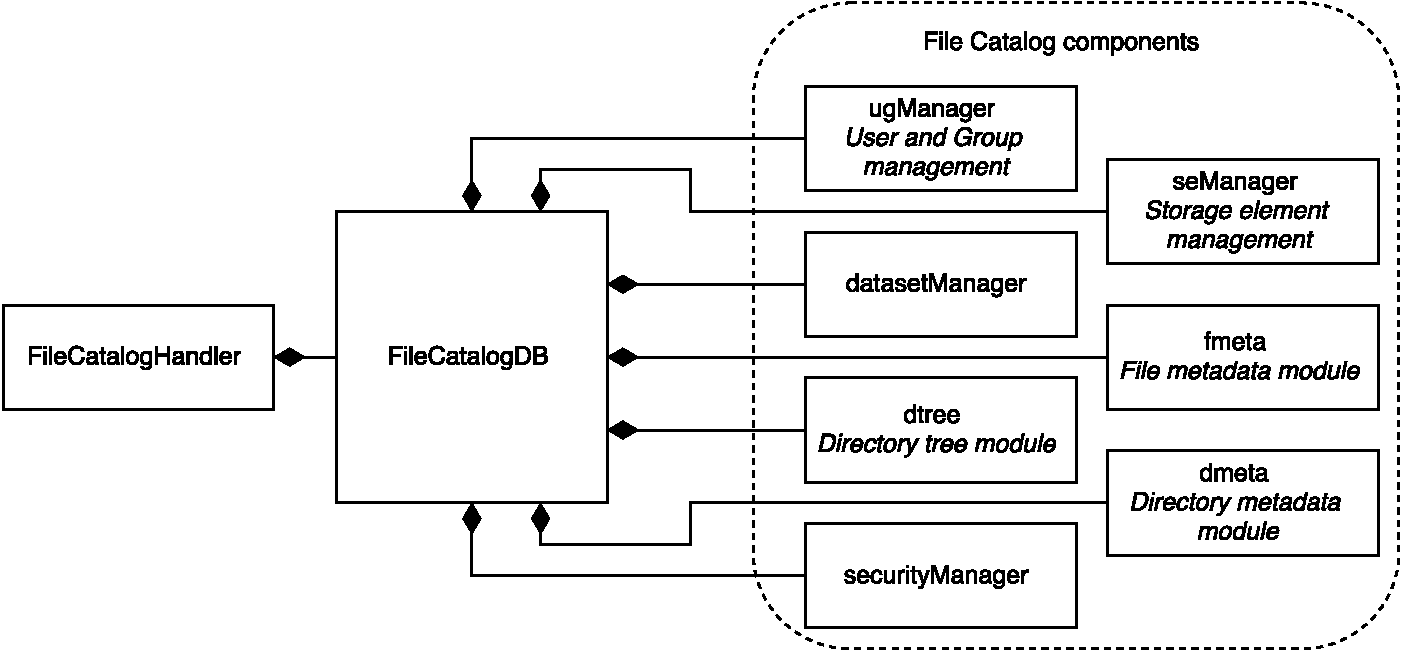
\includegraphics[width=\textwidth]{FCDB.pdf}
	\caption{Class diagram inside the File Catalog service. The clients requests are arriving at the 
	FileCatalogHandler class, the FileCatalogDB class then issues requests for MySQL database, sometimes using one
	or more of its' modules}
	\label{fig:FCClasses}
\end{figure}

\begin{figure}[b]
	\centering
	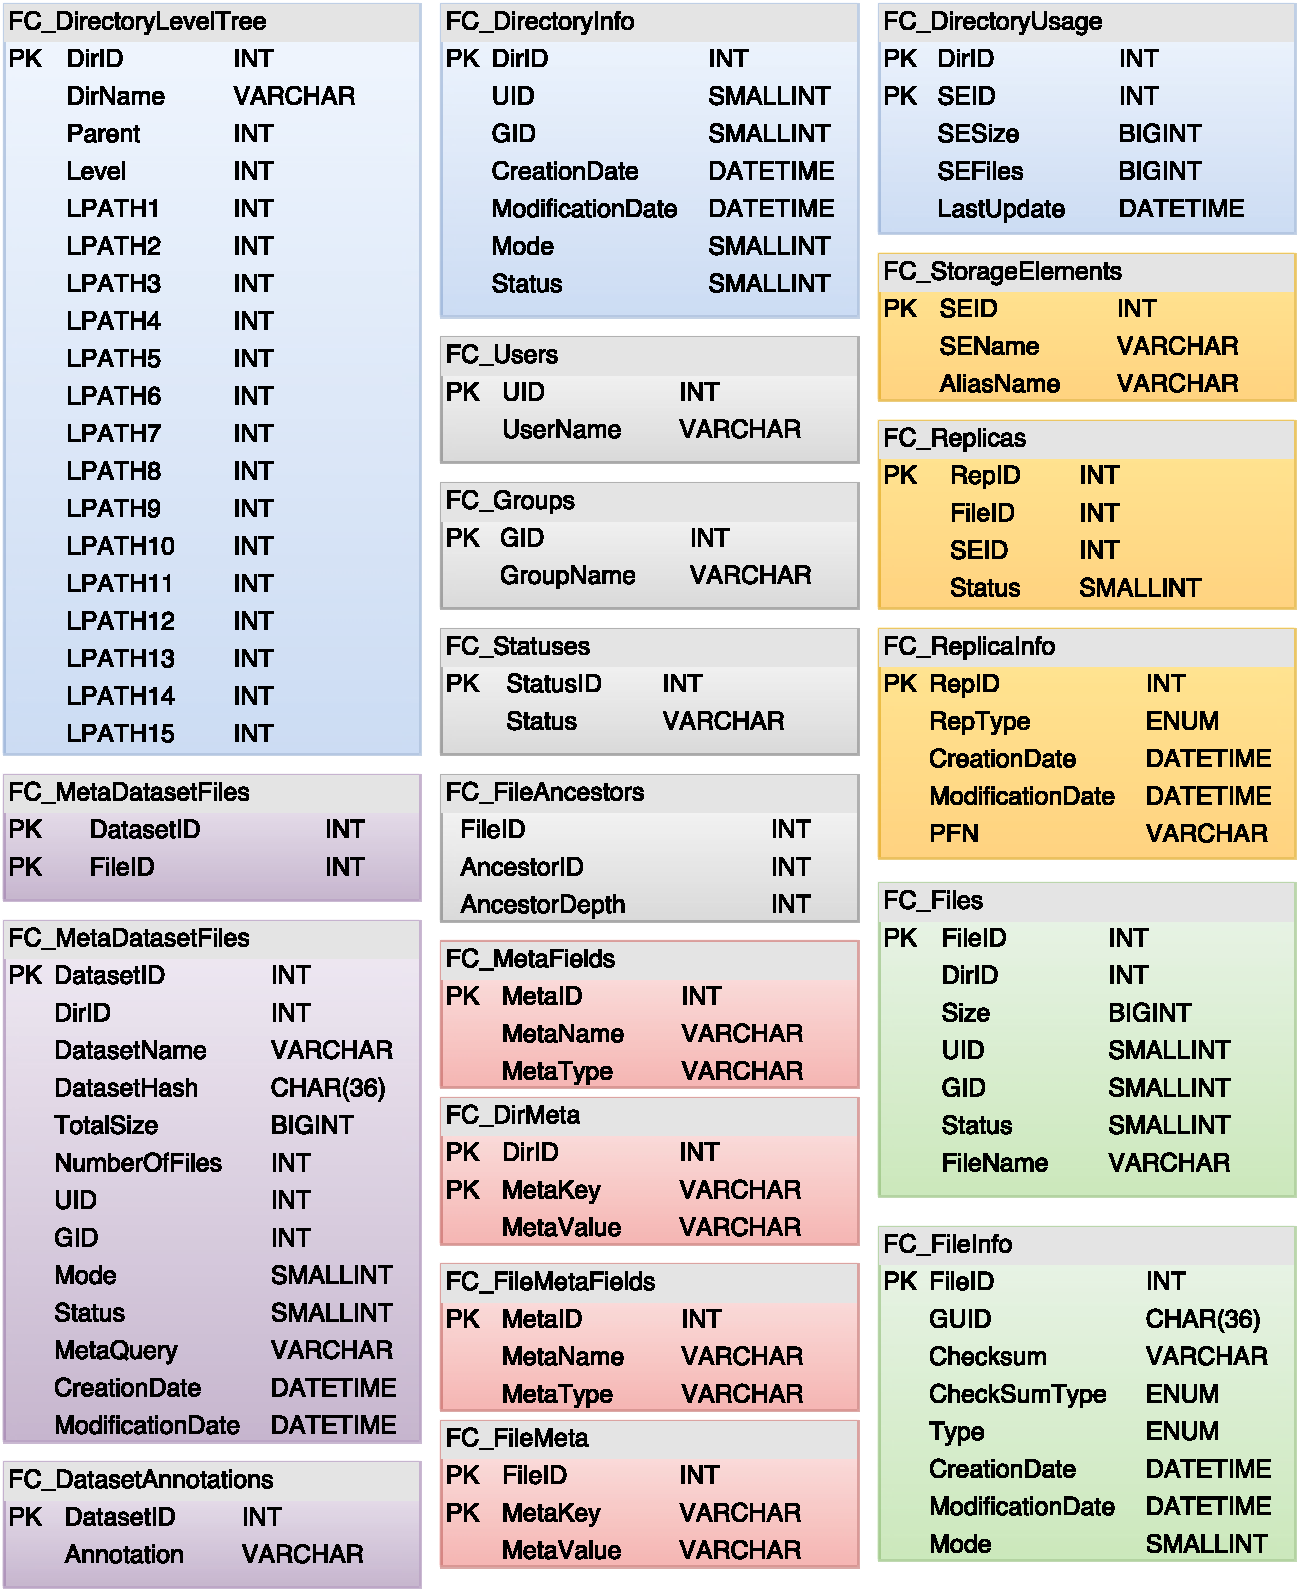
\includegraphics[width=\textwidth]{FCUML.pdf}
	\caption{UML diagram of the tables in the current MySQL implementation of the DIRAC File Catalogs DB. The color 
	scheme is chosen to make the orientation in the diagram easier: the grey tables are ``the core" of the File Catalog, blue are
	directory related, green are file related, purple are for the dataset manager, yellow are the Replica Catalog
	and red are the Metadata Catalog (in the initial state. When the user starts creating indexes, for each 
	index there is going to be a new table). Note that there are no relations between the tables, this is because
	no foreign keys are declared, all the table relationships are handled in DIRACs code.}
	\label{fig:FCMySQLUML}
\end{figure}

\subsection{DIRAC Replica Catalog}

When managing distributed storage systems, one of the major problems is how to translate the logical 
file name (LFN) into a URL of the file replicas, which in the DIRAC system is a task for the Replica
Catalog. The replica information can be stored in 2 different ways. In the first case, the full Physical File
Names (PFN) are stored as complete access URLs. In the second case, the DFC exploits a convention
that the PFNs are containing the corresponding LFNs as its trailing part. 
This helps to establish correspondence between the physical files and entries in the catalogs when checking 
the data integrity. There is also no need to store the full PFN in the catalog, when
the information about the wanted storage element (SE) is available. In such a case the PFN can be constructed on 
the fly and when the SE description changes, e.g. its access point, it is enough to change the SE description in the DIRAC 
Configuration System to continue receiving correct PFNs. Support for managing various user and group usage 
quotas is also implemented. Another feature supported by the Catalog based on the experience in 
the HEP\footnote{High Energy Physics} experiments is to store and provide information about ancestor-descendant 
relations between files. 

\subsection{Metadata Catalog}

Each virtual organization has varying needs in terms of file metadata, DIRAC takes this chance and 
attracts more users by enabling them to define their own. The Metadata Catalog keeps track of these 
arbitrary user metadata associated with his files and directories as key-value pairs. 
The catalog administrators can declare certain keys. In the current implementation whenever an 
index is being declared, another table in the MySQL database is created to store the values of the 
respective metadata. The indexed metadata can be used in file lookup operations. The value types include 
numbers, strings or time stamps. To decrease the amount of data in the database, and to simplify the 
administration, the metadata values are inherited in the directory structure. So when a metadata is 
associated with a directory, every file in the sub-tree with the root in this directory has the metadata
set as well. The directory hierarchy is common for both the Replica Catalog and the Metadata Catalog.

\subsection{DFC Interfaces}

The DFC is providing several user interfaces. The command \\ \texttt{dirac-dms-filecatalog-cli} launches a shell
connected to the file catalog the user is supposed to interact with, based on his or her user group and VO. Its 
functionality is similar to a classic UNIX shell, with commands like \texttt{ls, cd, chmod,...}, with added 
file catalog specific commands for handling metadata, replication, storage element usage reports.

The DFC Python API is a programming interface that allows creating any custom commands or even
small applications working on the DFC data.

The only graphical interface is provided by the Web portal. It features the DFC file browser
with a look and feel similar to desktop applications. %The DFC Web interface is built in the DIRAC 
%general Web Portal framework and provides a secure access based on the user certificates loaded into 
%the Web browser.
